\documentclass[a4paper,12pt]{article}

%%% Работа с русским языком
\usepackage{cmap}					% поиск в PDF
\usepackage{mathtext} 				% русские буквы в формулах
\usepackage[T2A]{fontenc}			% кодировка
\usepackage[utf8]{inputenc}			% кодировка исходного текста
\usepackage[english,russian]{babel}	% локализация и переносы
\usepackage{xcolor}
\usepackage{hyperref}
 % Цвета для гиперссылок
\definecolor{linkcolor}{HTML}{799B03} % цвет ссылок
\definecolor{urlcolor}{HTML}{799B03} % цвет гиперссылок

\hypersetup{pdfstartview=FitH,  linkcolor=linkcolor,urlcolor=urlcolor, colorlinks=true}

%%% Дополнительная работа с математикой
\usepackage{amsfonts,amssymb,amsthm,mathtools} % AMS
\usepackage{amsmath}
\usepackage{icomma} % "Умная" запятая: $0,2$ --- число, $0, 2$ --- перечисление

%% Номера формул
%\mathtoolsset{showonlyrefs=true} % Показывать номера только у тех формул, на которые есть \eqref{} в тексте.

%% Шрифты
\usepackage{euscript}	 % Шрифт Евклид
\usepackage{mathrsfs} % Красивый матшрифт

%% Свои команды
\DeclareMathOperator{\sgn}{\mathop{sgn}}
\pagestyle{empty}
%% Перенос знаков в формулах (по Львовскому)
\newcommand*{\hm}[1]{#1\nobreak\discretionary{}
{\hbox{$\mathsurround=0pt #1$}}{}}
% графика
\usepackage{graphicx}
\graphicspath{{pictures/}}
\DeclareGraphicsExtensions{.pdf,.png,.jpg}
\author{Бурмашев Григорий, БПМИ-208}
\title{}
\date{\today}
\begin{document}
{\Large \begin{center}
Бурмашев Григорий. 208. Матан -- 4
\end{center}}
\begin{center}
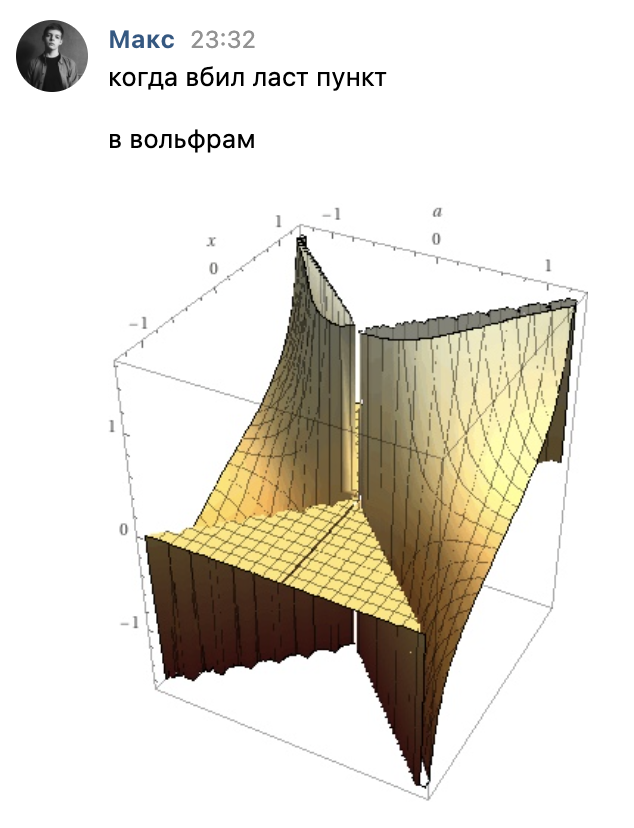
\includegraphics[scale=1]{a.png}
\end{center}
\begin{center}
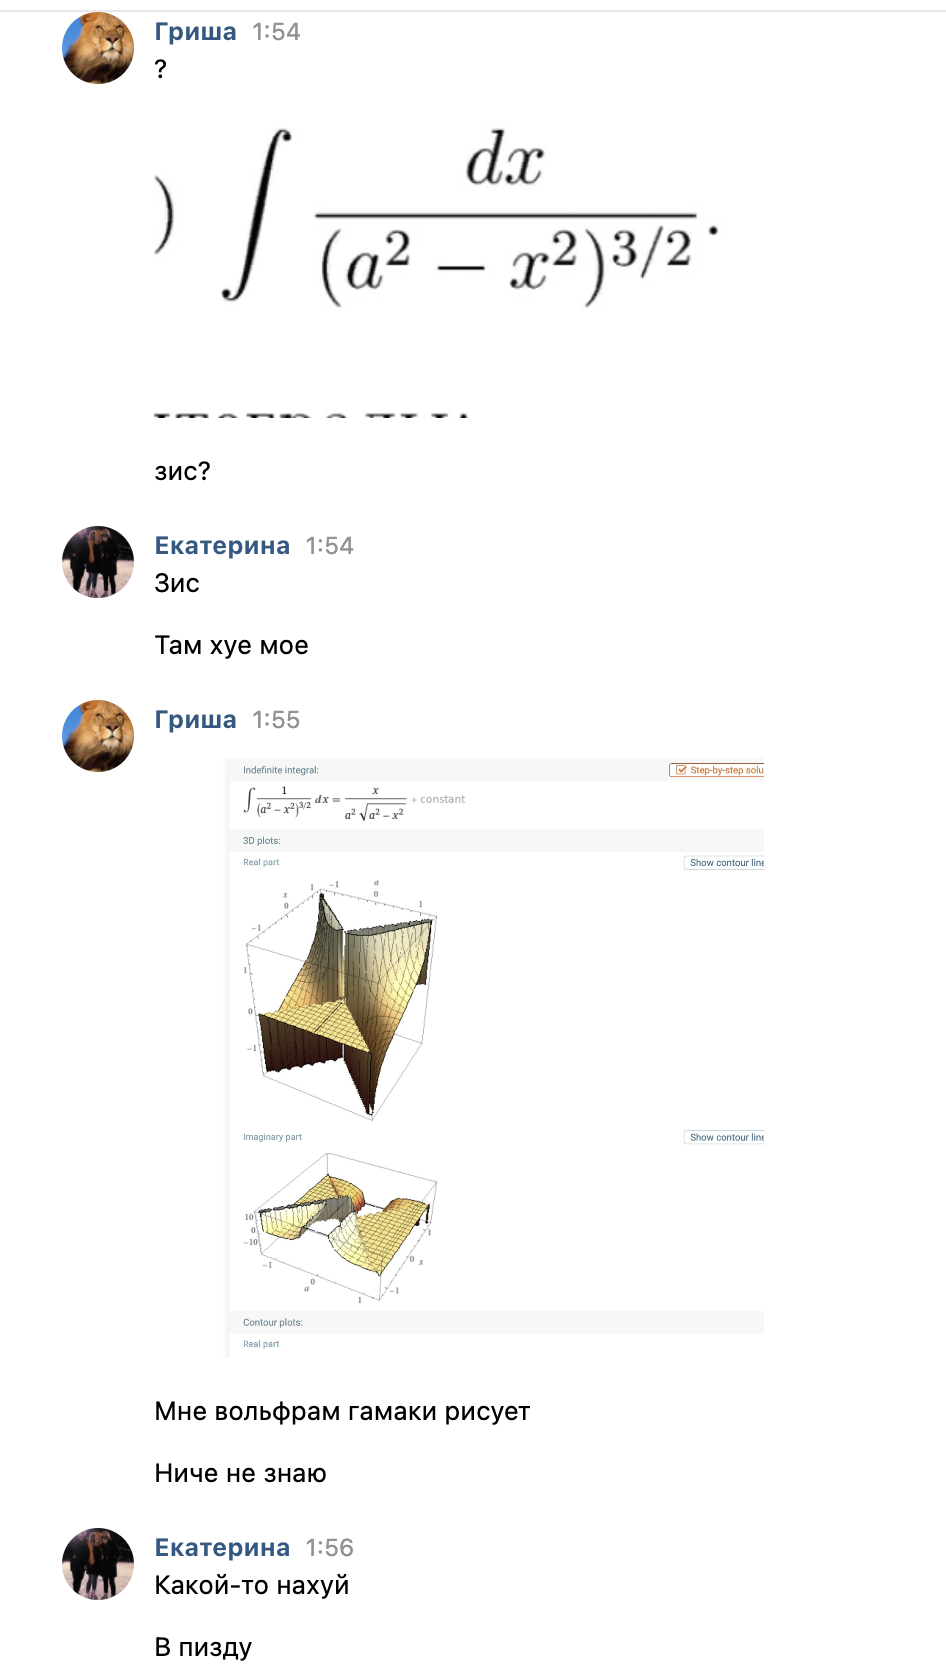
\includegraphics[scale=0.8]{e.png}
\end{center}
\clearpage
Пусть $C - \text{constant} $
\section*{Номер 6}
\subsection*{a)}
\begin{equation*}
\begin{gathered}
\int \frac{(x+1)^3}{x^2} \,dx = \int \frac{x^3 + 3x^2 + 3x + 1}{x^2} \,dx = \int x + 3 + \frac{3}{x} + \frac{1}{x^2} \,dx = \\
=
\frac{x^2}{2} + 3x + 3\ln |x| - \frac{1}{x} + C
\end{gathered}
\end{equation*}
{\Large \begin{center}
\textbf{Ответ: } $\frac{x^2}{2} + 3x + 3\ln |x| - \frac{1}{x} + C$
\end{center}}
\subsection*{b)}
\begin{equation*}
\begin{gathered}
\int \frac{1}{x^4-1} \,dx = \int \frac{1}{(x-1)(x+1)(x^2+1)} \,dx = \int \frac{a}{x-1)} + \frac{b}{x+1} + \frac{c}{x^2+1} \,dx \\
\\      
\begin{cases}
(x+1)(x^2+1) \cdot a + (x-1)(x^2+1) \cdot b + (x^2-1) \cdot c =  1 \\
(a+b)x^3 + (a+b)x + (a-b+c)x^2 + a  - b - c = 1
\end{cases} \\
\text{если x = -1, тогда 0a - 4b + 0c = 1} \\
\text{если x = 1, тогда 4a  + 0b  +0c = 1} \\
\text{если x = 0, тогда из второго условия } c =-\frac{1}{2}\\
\begin{cases}
a = \frac{1}{4} \\
b = -\frac{1}{4} \\
c = -\frac{1}{2} \\
\end{cases} \\
\int \frac{\frac{1}{4}}{x-1} + \frac{-\frac{1}{4}}{x+1} + \frac{-\frac{1}{2}}{x^2+1}\,dx = \frac{1}{4} \left[\ln |x-1| - \ln |x+1| - 2 \arctan x \right] + C \end{gathered}
\end{equation*}
{\Large \begin{center}
\textbf{Ответ: } $\frac{1}{4} \left[\ln |x-1| - \ln |x+1| - 2 \arctan x \right] + C $
\end{center}}
\subsection*{c)}
\begin{equation*}
\begin{gathered}
\int  \frac{2^{2x-1} - 3^{2x+2}}{6^{2x}} \,dx = \int \left[ \frac{1}{2} \cdot 9^{-x} - 9 \cdot 4^{-x} \right] \,dx = -\frac{9^{-x}}{2 \ln 9} + \frac{9 \cdot 4^{-x}}{\ln 4} + C
\end{gathered}
\end{equation*}
{\Large \begin{center}
\textbf{Ответ: } $-\frac{9^{-x}}{2 \ln 9} + \frac{9 \cdot 4^{-x}}{\ln 4} + C$
\end{center}}
\subsection*{d)}
\begin{equation*}
\begin{gathered}
\int \frac{e^{3x} - 1}{e^x - 1} \, dx = \int \frac{(e^x -1)(e^{2x} + e^x + 1)}{e^x -1} \,dx = \int \left[e^{2x} + e^x + 1\right] \,dx = \frac{e^{2x}}{2} + e^x +  x + C
\end{gathered}
\end{equation*}
{\Large \begin{center}
\textbf{Ответ: } $\frac{e^{2x}}{2} + e^x +  x + C$
\end{center}}
\subsection*{e)}
\begin{equation*}
\begin{gathered}
\int \frac{1}{\sin^2 x \cdot cos^2 x} \,dx = \int \frac{4}{\sin^2 \left( 2x\right)} \,dx = - 2 \text{ctg} \left(2x\right) + C
\end{gathered}
\end{equation*}
{\Large \begin{center}
\textbf{Ответ: } $- 2 \text{ctg} \left(2x\right) + C$
\end{center}}
\subsection*{f)}
\[
\int \frac{1}{\cos x + \sin x} \,dx
\]
Воспользуемся универсальной тригонометрической подстановкой (хз было ли это у нас но мне зашарили XD):

Пусть:
\[
\cos x = \frac{1 - tg^2 \frac{x}{2}}{1 + tg^2 \frac{x}{2}}
\]
\[
\sin x = \frac{2 tg \frac{x}{2}}{1 + tg^2 \frac{2}{2}}
\]
Тогда:
\[
t = tg \frac{x}{2}, dx = \left[\frac{2}{1 + t^2} \right]dt
\]
Возвращаемся:
\[
\int \left[ \frac{1}{\frac{1 - t^2}{1 + t^2} +\frac{2t}{1 + t^2}} \right]\left[\frac{2}{1 + t^2} \right]dt =\int \left[ \frac{2}{-t^2 + 2t+ 1} \right] dt = 2 \cdot \int \frac{1}{(-t^2 +2t +1)} dt = 
\]
\[
= 2 \int \frac{1}{(2 - (t-1)^2)}dt 
\]
Пусть $ s = t -1$, $ds = dt$:
\[
2 \int \frac{1}{2 - s^2} ds = 2 \cdot \frac{1}{2} \int \frac{1}{1 - \frac{s^2}{2}} ds 
\]
Пусть $ u = \frac{s}{\sqrt{2}}$,  $du = \frac{ds}{\sqrt{2}}$:
\[
\sqrt{2} \int \frac{1}{1 - u^2} du =  \sqrt{2} \cdot \frac{1}{2} (\ln(u + 1) - \ln(u-1))  + C= \frac{\ln ( t + \sqrt{2} -1) - \ln(-t + \sqrt{2} + 1)}{\sqrt{2}} + C= 
\]
\[
= \frac{\ln ( tg \frac{x}{2} + \sqrt{2} -1) - \ln(-tg \frac{x}{2} + \sqrt{2} + 1)}{\sqrt{2}} + C=  \frac{\ln \left(\frac{\ln ( tg \frac{x}{2} + \sqrt{2} -1) }{\ln(-tg \frac{x}{2} + \sqrt{2} + 1)}\right)}{\sqrt{2}} + C
\]
{\Large \begin{center}
\textbf{Ответ: } $ \frac{\ln \left(\frac{tg \frac{x}{2} + \sqrt{2} -1}{\-tg \frac{x}{2} + \sqrt{2} + 1}\right)}{\sqrt{2}} + C$ 
\end{center}}
\section*{Номер 7}
\subsection*{a)}
\[
\int x \cdot \sin (x^2) \,dx
\]
Пусть $x = t^2$, $x = \sqrt{t}$, $dx = \frac{dt}{2\sqrt{t}}$
\[
\int \sqrt{t} \cdot \sin (t) \frac{dt}{2\sqrt{t}} =  \int \frac{\sin t}{2} dt = -\frac{\cos(t)}{2} + C = -\frac{\cos(x^2)}{2} + C\]
{\Large \begin{center}
\textbf{Ответ: } $ -\frac{\cos(x^2)}{2} + C$
\end{center}}
\subsection*{b)}
\[
\int \frac{e^x + e^{2x}}{1-e^x} \,dx
\]
Пусть $e^x = t$, $dx = \frac{dt}{t}$
\[
\int\left[ \frac{t + t^2}{1 - t} \cdot \frac{1}{t}  \right]dt= \int \frac{t(t+1)}{(1-t)t} dt = \int \frac{t+1}{1-t}dt = \int (\frac{t}{1-t} + \frac{1}{1-t}) dt  =
\]
\[
= - \ln |t - 1| - \int \left(1 + \frac{1}{t-1}\right) dt = -2 \ln \left( |t - 1| \right) - t+ C = 
\]
\[
-2 \ln \left( |e^x - 1| \right) - e^x + C
\]
{\Large \begin{center}
\textbf{Ответ: } $-2 \ln \left( |e^x - 1| \right) - e^x + C$
\end{center}}
\subsection*{c)}
\[
\int \frac{dx}{x(\ln x + 5)}
\]
Пусть $t = \ln x$, $x = e^t$, $dx = e^t\cdot dt$, тогда x сократится:
\[
\int \frac{e^t}{e^t\cdot (t+5)} dt= \int \frac{dt}{t+5} = \ln |t+5|+ C = \ln \left(|\ln x + 5|\right) + C
\]
{\Large \begin{center}
\textbf{Ответ: } $\ln \left(|\ln x + 5|\right) + C$
\end{center}}
\subsection*{d)}
\[
\int \frac{1}{\cos x} \,dx = \int  \frac{\cos x}{\cos^2 x} \,dx = \int \frac{\cos x}{(1 - \sin^2 x)} \,dx
\]
Пусть $t = \sin x$, $dx = \frac{dt}{\cos x}$
\[
\int \left[\frac{\cos x}{(1-t)(1+t)} \cdot \frac{1}{\cos x} \right]dt=  \int \frac{dt}{(1-t)(1+t)} = \frac{1}{2} \cdot \left(\ln |t + 1| - \ln |t-1|\right) + C =
\]
\[
= \frac{1}{2} \cdot \ln \left(
\left |\frac{\sin x + 1}{\sin x - 1}\right|\right ) + C
\]
{\Large \begin{center}
\textbf{Ответ: } $\frac{1}{2} \cdot \ln \left(
\left |\frac{\sin x + 1}{\sin x - 1}\right|\right ) + C
$
\end{center}}
\subsection*{e)}
\[
\int  \frac{\sin (2x) } { \sqrt{1 - 4 \sin^2x}} \,dx = \int  \frac{2 \sin x \cos x } { \sqrt{(1-2\sin x)(1 + 2 \sin x)}}\,dx
\]
Пусть $t = 2 \sin x $, $dx = \frac{dt}{2 \cos x}$
\[
\int \left[ \frac{2t \cdot cos x}{2\sqrt{(1-t)(1+t)}} \cdot \frac{1}{2 \cos x} \right] dt = \int \frac{dt}{2\sqrt{1-t^2}} = 
\]
\[
=
-\frac{\sqrt{1-t^2}}{2} + C = -\frac{\sqrt{1-4\sin^2 x }}{2} + C
\]
{\Large \begin{center}
\textbf{Ответ: } $ -\frac{\sqrt{1-4\sin^2 x }}{2} + C$
\end{center}}
\subsection*{f)}
\[
\int \sin^7 x \,dx = \int \sin x \cdot \sin^6 x \,dx = \int \sin x \cdot (1-\cos^2 x)^3 \,dx
\]
Пусть $t = \cos x$, $dx = -\frac{dt}{\sin x}$
\[
\int \left[ \sin x \cdot (1 -t^2)^3 \cdot \left(-\frac{1}{\sin x} \right) \right]dt  = \int -(1-t^2)^3 \,dt  = \int (t^2-1)^3 dt =  
\]
\[
= \int (t^2 - 2t + 1)^3 dt = \int(t^6 - 3t^4 + 3t^2 -1) dt = \frac{t^7}{7} - 3\cdot \frac{t^5}{5} + t^3 - t + C = 
\]
\[
= \frac{\cos^7 x}{7} - \frac{3 \cos^5 x}{5} + \cos^3 x - \cos x + C
\]
{\Large \begin{center}
\textbf{Ответ: } $\frac{\cos^7 x}{7} - \frac{3 \cos^5 x}{5} + \cos^3 x - \cos x + C$
\end{center}}
\subsection*{g)}
\[
\int x^2 \cdot \sqrt{1-x^2} \,dx
\]
Пусть $ x = \sin t $, $dx = \cos t \; dt$, $  t = \text{arcsin} x$
\[
\int \sin^2 t \cdot \sqrt{1 - \sin^2t} \cdot \cos t\; dt = \int \sin^2 t \cdot \cos t \cdot \cos t \; dt =А
\]
\[
=
\int (\sin^2 t \cdot cos^2 t) dt = \int \frac{\sin^2 (2t)}{4} dt = \int \frac{1- \cos 4t}{8} dt = \frac{1}{8} \cdot \int (1-\cos 4t) dt = 
\]
\[
= \frac{ \text{arcsin} }{8} - \frac{\sin \left( 4 \text{arcsin}x\right)}{8 \cdot 4} + C = \frac{ \text{arcsin} }{8} - \frac{\sin \left( 4 \text{arcsin}x\right)}{32} + C
\]
{\Large \begin{center}
\textbf{Ответ: } $\frac{ \text{arcsin} }{8} - \frac{\sin \left( 4 \text{arcsin}x\right)}{32} + C$
\end{center}}
\subsection*{h)}
\[
\int \frac{dx}{(a^2 - x^2)^{\frac{3}{2}}} \,dx
\]
Пусть $x = a \cdot \sin t$, $ t = \text{arcsin} \frac{x}{|a|}$, $dx = a \cdot \cos t \; dt$

Тогда $(a^2 - x^2)^\frac{3}{2} = (a^2 - a^2 \sin^2 t)^\frac{3}{2} = |a^3| \cdot |\cos^3 t|$
\[
\int \frac{a \cdot \cos t \; dt}{|a^3| \cdot |\cos^3 t} = \frac{1}{a^2} \int \frac{1}{\cos^2 t} dt = \frac{\tg \left(\text{arcsin} \left(\frac{x}{|a|}\right)\right)}{a^2} + C
\]
{\Large \begin{center}
\textbf{Ответ: } $\frac{\tg \left(\text{arcsin} \left(\frac{x}{|a|}\right)\right)}{a^2} + C$
\end{center}
\end{document}
